\section{Closure and Persistent Structure}
\label{sec:closure}

\subsection{What Is Closure}

A \textbf{closure} is a configuration in which causal flow circulates along
a loop, the loop reinforces itself through the self-referential selection
equation~\cref{eq:Cij}, and the resulting pattern is dynamically sustained.
A closure is not a boundary, but a circulation that sustains itself.

Without closure, flows dissipate.
With closure, flow is trapped, gradients are maintained, and structure persists.

\subsection{The Minimal Closure Is Triangular}

The minimal loop that admits nontrivial closure must involve at least
three nodes:

\begin{itemize}
  \item \textbf{Two nodes}: the only cycle $i \to j \to i$ is purely
    oscillatory, with no internal degrees of freedom and no stable phase
    structure.
  \item \textbf{Three nodes}: the cycle $i \to j \to k \to i$ admits an
    oriented loop with internal area. The three edges span a two-dimensional
    phase space, allowing stable phase relationships.
  \item \textbf{Four or more}: any such cycle decomposes into triangular
    sub-loops. No new topological structure is introduced.
\end{itemize}

\begin{keybox}
\textit{The minimal closure is triangular.
This is a topological result, not an assumption.}
\end{keybox}

\subsection{Closure as a Dynamical Attractor}

Define the \textbf{closure energy} of a configuration $A$:

\begin{equation}
  E(A)
  = \alpha\left|\sum_{i\in A}\vec{e}_i\right|^2
  - \beta\,\Phi(A)
  + \gamma|A|
  + B(L(A)),
  \label{eq:closure_energy}
\end{equation}

where $\vec{e}_i$ are internal flux vectors derived from $C_{ij}$,
$\Phi(A) = \sum_{i<j<k\in A}\phi_{ijk}$ is the non-degeneracy measure,
and $B(L)$ is the closure barrier of \cref{eq:barrier}.

\begin{definition}
A \textbf{particle} is a local minimum of the closure energy $E(A)$.
\end{definition}

\subsection{Closure Distance and Mass}

The \textbf{closure distance} of a stable configuration:

\begin{equation}
  \Delta_k = L_{\max} - L_k
  \label{eq:delta}
\end{equation}

measures how far the configuration is from complete closure.
The curvature of $E$ at the minimum gives the effective mass:

\begin{keybox}
\begin{equation}
  m_k
  \propto \left.\frac{d^2 E}{dL^2}\right|_{L_k}
  \sim \frac{\kappa_B}{\Delta_k^2}.
  \label{eq:mass}
\end{equation}
\end{keybox}

\begin{keybox}
\textit{Heavy structures sit close to the complete-closure limit.
The world is made of incomplete closures.}
\end{keybox}

This minimal structure is illustrated in Fig.~\ref{fig:triangular_closure}.

\begin{figure}[t]
\centering
\setcounter{figure}{2}
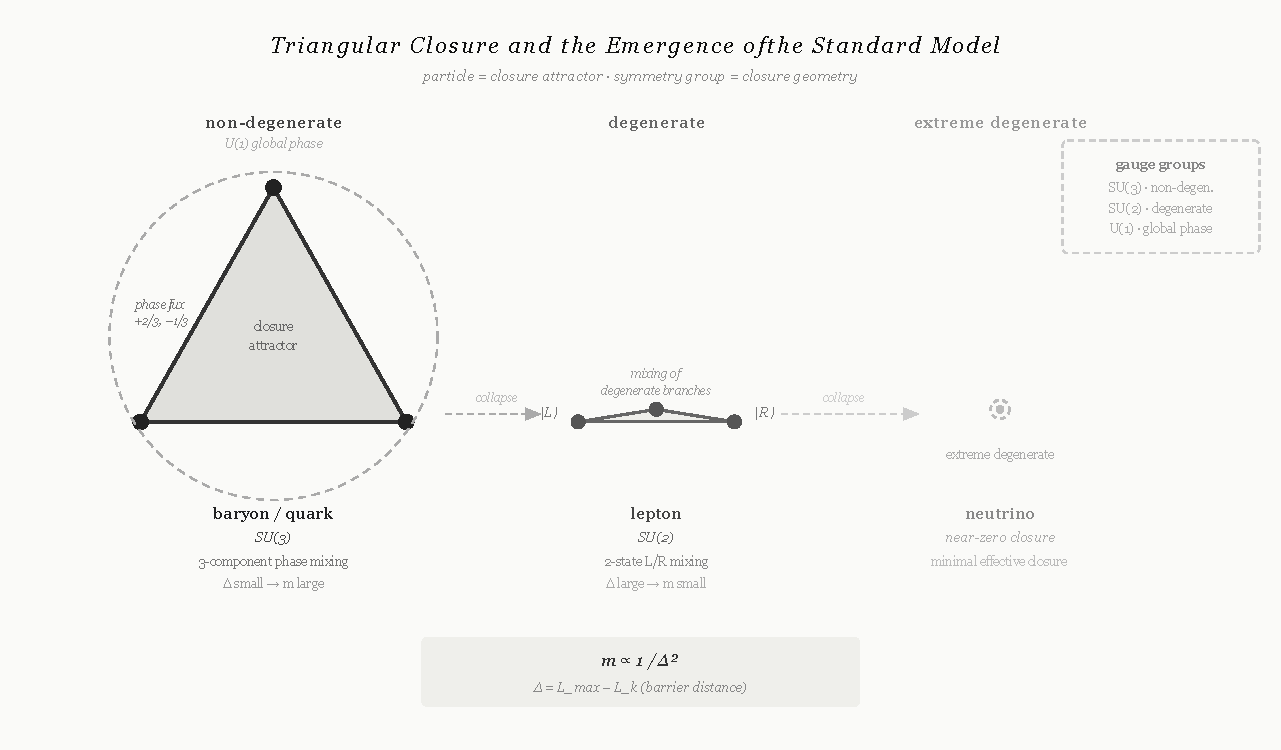
\includegraphics[width=0.6\linewidth]{figures/fig3_triangular_closure.pdf}
\caption{
Triangular closure types and their correspondence to particle families.
The three configurations illustrate non-degenerate, degenerate, and extreme degenerate closures
as the simplest persistent enclosures, forming the basis for higher-order symmetries explored in subsequent work.
}
\label{fig:triangular_closure}
\end{figure}
